%!TEX root = main.tex
%!TEX encoding = UTF-8 Unicode

\appendix

\part{Appendix 附录}
\chapter[矢量代数]{Vector calculus 矢量代数}\label{appendix.A}
物理中常用三个数$ \begin{pmatrix}
x \\ y \\ z
\end{pmatrix}$来描述一个东西的位置。我们将其称作矢量$\vec{v}$,在它头上放了一个箭头。这三个数称作矢量沿三个坐标轴的分量。第一个数说了这个矢量沿$x$方向走了多远,第二个是沿$y$方向以及第三个是沿$z$方向。例如,$\vec{w}= \begin{pmatrix}
0 \\ 4 \\ 0
\end{pmatrix}$是一个指向$y$轴方向的矢量。

\marginpar{
	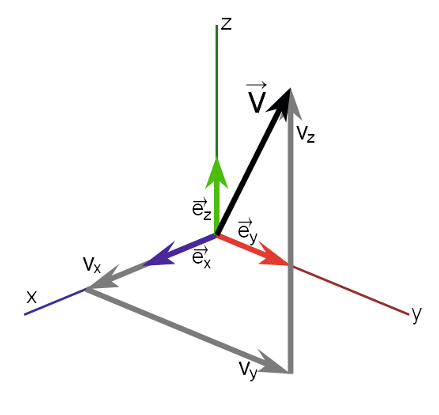
\includegraphics[width=.4\textwidth]{./../Pictures/fig_appendix_A_1.png}
}

矢量间可以相加
\begin{equation}
\vec{v} = \begin{pmatrix}
v_x \\ v_y \\ v_z
\end{pmatrix} \quad
\vec{w} = \begin{pmatrix}
w_x \\ w_y \\ w_z
\end{pmatrix} \quad \rightarrow \quad
\vec{v}+\vec{w}= \begin{pmatrix}
v_x+w_x \\ v_y+w_y \\ v_z+w_z
\end{pmatrix}
\end{equation}
也可以相乘
\begin{equation}
\vec{v}\cdot\vec{w} = \begin{pmatrix}
v_x \\ v_y \\ v_z
\end{pmatrix} \cdot \begin{pmatrix}
w_x \\ w_y \\ w_z
\end{pmatrix} =
v_xw_x +v_yw_y +v_zw_z\text{。}
\end{equation}

乘法的结果是一个数($=$标量)而不是矢量,其有特定的名称:{标量积(scalar product)}。计算矢量与自身的标量积可以得到其长度:
\begin{equation}
\text{长度}(\vec{v}) = \sqrt{\vec{v}\cdot\vec{v}}\text{。}
\end{equation}
注意并不是随便三个量都可以写在一起,用括号包起来,作为一个矢量。例如,把一个房间里的温度$T$,压强$P$和湿度$H$放在一起:
\begin{equation}
\begin{pmatrix}
T \\ P \\ H
\end{pmatrix}\text{。}
\end{equation}
没人阻止我们把他们放在一起,但这结果毫无意义,而且显然不是一个矢量,因为不存在能将它们混在一起的线性关系。而如果我们仅仅是换一个视角\footnote{译注:本意,即视线的角度。}去考察一个矢量,它的坐标分量将会互相转换%
\mpar{这一点等会儿会有更清楚的说明。}%
。故将这些坐标分量写在一起用括号包起来是有用的。另外,如果分量会因视角的改变而发生混合的话,将其写成位置矢量的形式是有用的。

从现在开始,我们将完全按照位置矢量$\vec{v}$的变换方式的量称为一个矢量。这句话的意思是,如果在某种变换下我们有$\vec{v}\rightarrow\vec{v}'=M\vec{v}$,则任何依$\vec{w}\rightarrow\vec{w}'=M\vec{w}$作变换的量都是矢量。动量和加速度是典型的例子。

物理中我们将经常碰到这种思路。当我们把一些量写在一起放在一对括号中时,它们未必是矢量,但一定是在某些线性算符下相互变换的量。线性算符常通过与矩阵的乘法来表示。

\section[基矢]{Basis Vectors 基矢}\label{appendix.A.1}
我们可以通过引入基矢来更一般的讨论沿坐标轴的分量这件事。基矢是一组线性独立%
\mpar{一组矢量$\{\vec{a},\vec{b},\vec{c}\}$被称为是线性独立的,若方程$c_1\vec{a}+c_2\vec{b}+c_3\vec{c}=0$成立当且仅当$c_1=c_2=c_3=0$。这说的其实就是其中任何一个矢量不能表达为其他矢量的线性组合:如果有$c_1\vec{a}+c_2\vec{b}+c_3\vec{c}=0$对非零的系数成立,则有$c_1\vec{a}+c_2\vec{b}=-c_3\vec{c}$。}%
且长度为一%
\footnote{译注:一般资料上并不要求最后一条;满足这一条的称为单位基矢。}%
的矢量。三维里我们需要三个基矢,从而能将任何矢量都用基矢量的组合来表达。一个简单的选择是:
\begin{equation}
\vec{e}_1 = \begin{pmatrix}
1 \\ 0 \\ 0
\end{pmatrix}\text{,}\quad
\vec{e}_2 = \begin{pmatrix}
0 \\ 1 \\ 0
\end{pmatrix} \text{,}\quad
\vec{e}_3 = \begin{pmatrix}
0 \\ 0 \\ 1
\end{pmatrix}
\end{equation}
这样任意三维矢量$\vec{v}$都能用基矢表出
\begin{equation}
\vec{v} = \begin{pmatrix}
v_x \\ v_y \\ v_z
\end{pmatrix} = v_1\vec{e}_1 + v_2\vec{e}_2 + v_3\vec{e}_3 =
v_1 \begin{pmatrix}
1 \\ 0 \\ 0
\end{pmatrix}+
v_2  \begin{pmatrix}
0 \\ 1 \\ 0
\end{pmatrix} +
v_3  \begin{pmatrix}
0 \\ 0 \\ 1
\end{pmatrix}\text{。}
\end{equation}
$v_1,v_2,v_3$三个数叫做$\vec{v}$的分量。注意分量是依赖于基矢的。

前面提到的矢量\mpar{$\vec{w}= \begin{pmatrix}
0\\4\\0
\end{pmatrix}$}$\vec{w}$由此可以写成$\vec{w}= 0\vec{e}_1 + 4\vec{e}_2 + 0\vec{e}_3$。对基矢另一个同样好的选法是
\begin{equation}
\tilde\vec{e}_1 = \frac{1}{\sqrt{2}} \begin{pmatrix}
1 \\ 1 \\ 0
\end{pmatrix}\text{,}\quad
\tilde\vec{e}_2 = \frac{1}{\sqrt{2}} \begin{pmatrix}
1 \\ -1 \\ 0
\end{pmatrix} \text{,}\quad
\tilde\vec{e}_3 = \begin{pmatrix}
0 \\ 0 \\ 1
\end{pmatrix}\text{。}
\end{equation}
在这组基下矢量$\vec{w}$看起来会有点不同:
\begin{equation}
\vec{w}= 2\sqrt{2}\tilde\vec{e}_1 -2\sqrt{2}\tilde\vec{e}_2 + 0\tilde\vec{e}_3
= 2\sqrt{2} \frac{1}{\sqrt{2}} \begin{pmatrix}
1 \\ 1 \\ 0
\end{pmatrix}-2\sqrt{2}
\frac{1}{\sqrt{2}} \begin{pmatrix}
1 \\ -1 \\ 0
\end{pmatrix} =\begin{pmatrix}
0\\4\\0
\end{pmatrix} \text{。}
\end{equation}
从而将$\vec{w}$用在新基矢下的分量写出
\[
\tilde\vec{w} = \begin{pmatrix}
2\sqrt{2} \\ -2\sqrt{2} \\ 0
\end{pmatrix}\text{。}
\]
这并不是一个不同的矢量,而只是一个不同的描述!准确地讲,$\tilde\vec{w}$是原坐标系中的矢量$\tilde\vec{w}$在一个相对有旋转的坐标系下描述。%
\footnote{译注:在整个附录\ref{appendix.A}里作者就没说过几句准确的话,这句话也说得挺糙的。}

\section[坐标系变换]{Change of Coordinate Systems 坐标系变换}\label{appendix.A.2}
通过矩阵,我们可以更精确地描述不同坐标系间的联系。两个不同的坐标系可以代表实验中两个持不同视角的观察者,或者仅仅是{\bf 一个}想使用一套新的基矢的观察者。这些描述之间的关系是什么?为了避免复杂的讨论,让我们假定这两个坐标系的原点和$z$轴都是一样的。这样的话就只是$x$和$y$轴有区别了。进一步假定实验中某个重要的量用矢量$\vec{v}$描述。

如果第一个观察者看到的是矢量$\vec{v}= \begin{pmatrix}
v_x \\ v_y \\ v_z
\end{pmatrix}$,我们能通过三角函数$\sin(\phi)$,$\cos(\phi)$和$\tan(\phi)=\frac{\sin(\phi)}{\cos(\phi)}$来计算出第二个观察者看到的$\vec{v}= \begin{pmatrix}
v_{x'} \\ v_{y'} \\ v_{z'}
\end{pmatrix}$,如图\ref{fig:appendix.A.1} 所示:
\marginpar{
	\figcaption{矢量在两个不同的坐标系下分量的示意图。细节见正文。}
	\label{fig:appendix.A.1}
}

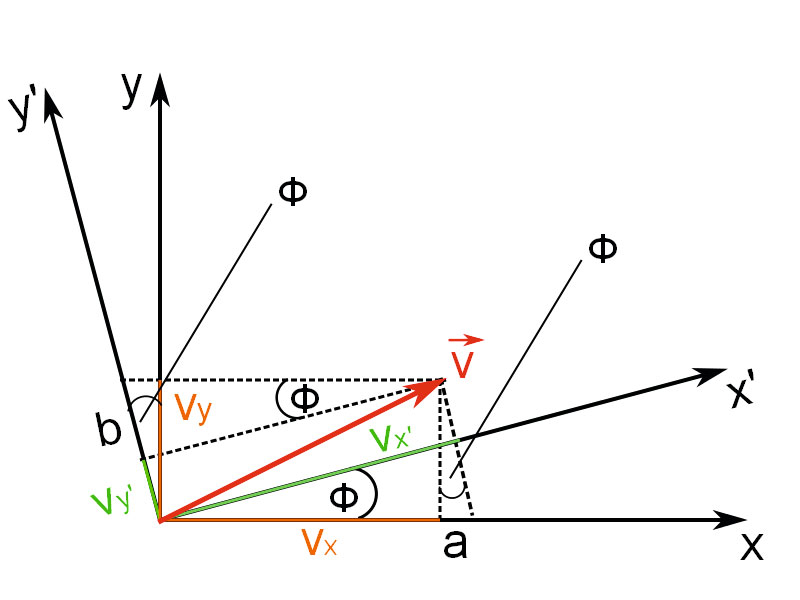
\includegraphics[width=\textwidth]{./../Pictures/fig_appendix_A_3.png}

计算$v_x$和$v_{x'}$的关系,由
\[
\cos(\phi)=\frac{v_{x'}}{v_x+a} \rightarrow v_{x'}=(v_x+a)\cos(\phi)
\]
以及
\[
\tan(\phi)=\frac{a}{v_y}\rightarrow a=v_y\tan(\phi)\text{。}
\]
得到
\[
\begin{aligned}
v_{x'}=(v_x+v_y\tan(\phi))\cos(\phi)&=\left(v_x+v_y\frac{\sin(\phi)}{\cos(\phi)}\right)\cos(\phi) \\
 & = v_x\cos(\phi)+v_y\sin(\phi)\text{。}
\end{aligned}
\]
类似的,利用
\[
\cos(\phi) = \frac{v_y}{v_{y'}+b}\rightarrow v_{y'}=v_y\frac{1}{\cos(\phi)}-b
\]
和
\[
\tan(\phi)=\frac{v_y}{v_{y'}+b}\rightarrow b=v_{x'}\tan(\phi)
\]
再借助$\sin^2(\phi)+\cos^2(\phi)=1$导出
\[\begin{split}
v_{y'}&=v_y\frac{1}{\cos(\phi)}-v_{x'}\tan(\phi)=v_y\frac{1}{\cos(\phi)}-(v_x\cos(\phi)+v_y\sin(\phi))\frac{\sin(\phi)}{\cos(\phi)}  \\
&= v_y\frac{\sin^2(\phi)+\cos^2(\phi)}{\cos(\phi)}-v_x\sin(\phi)-v_y\frac{\sin^2(\phi)}{\cos(\phi)} = v_y\cos(\phi)-v_x\sin(\phi)
\end{split}\]
最终有$v_{y'}=-v_x\sin(\phi)+v_y\cos(\phi)$。

我们能将其用一个旋转矩阵来表达:
\begin{equation}
\begin{aligned}
\begin{pmatrix}
v_{x'} \\ v_{y'} \\ v_{z'}
\end{pmatrix} &= R_z(\phi)\vec{v} =
\begin{pmatrix}
\cos(\phi) & \sin(\phi) & 0 \\
-\sin(\phi) & \cos(\phi) & 0 \\
0 & 0 & 1
\end{pmatrix}
\begin{pmatrix}
v_x \\ v_y \\ v_z
\end{pmatrix} \\
&= \begin{pmatrix}
\cos(\phi)v_x+\sin(\phi)v_y \\ -\sin(\phi)v_x+\cos(\phi)v_y \\ v_z
\end{pmatrix}\text{。}
\end{aligned}
\end{equation}
将矩阵的每一行与未旋转的矢量相乘,便得到了旋转后的矢量。如之前所提到的,沿$z$轴的分量$v_3$对于不同的观察者而言是相同的。矩阵$R_z(\phi)$描述了一个绕$z$轴转动了角度$\phi$的旋转。

\section[矩阵乘法]{Matrix Multiplication 矩阵乘法}\label{appendix.A.3}
像这样通过矩阵来作计算是一个极大的简化。矩阵乘法的规则就是行乘列。如果将一个矢量看做一个一列三行的矩阵(一个$3\times 1$矩阵),则标量积也可以看做是矩阵乘法的一种特殊情况。即
\begin{equation}
\vec{v}\cdot\vec{w} = \vec{v}^T\vec{w}= \begin{pmatrix}
v_x & v_y & v_z
\end{pmatrix} \begin{pmatrix}
w_x \\ w_y \\ w_z
\end{pmatrix} = v_xw_x +v_yw_y +v_zw_z\text{,}
\end{equation}
其中$T$代表转置,即行变成列,列变成行。那么$\vec{v}^T$便是一个$1$行$3$列的矩阵。这样写的话标量积就也成了行乘列的矩阵乘法。

类似的,两个矩阵的乘法也就是左边矩阵的每一行乘右边矩阵的每一列,如图\ref{fig:appendix.A.2}。下面是一个具体的例子

\marginpar{
	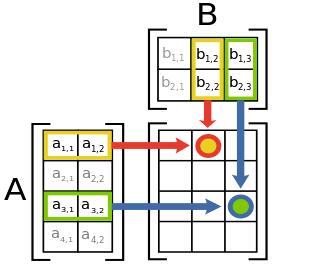
\includegraphics[width=.4\textwidth]{./../Pictures/fig_appendix_A_4.png}
	\figcaption{矩阵乘法示意图。时时刻刻记住{\bf 行乘列}。第一个指标代表所在的行数,第二个代表列数。在例子中,乘积矩阵红色的元素$c_{1,2}=a_{1,1}b_{1,2}+a_{1,2}b_{2,2}$,蓝色的元素$c_{3,3}=a_{3,1}b_{1,3}+a_{3,2}b_{2,3}$。一般的,$c_{i,j}=a_{i,k}b_{k,j}=a_{i,1}b_{1,j}+a_{i,2}b_{2,j}+\dots$ Figure by Olivier Perrin (Bilou Wikimedia Commons) released under a CC BY-SA 3.0 licence: \url{http://creativecommons.org/licenses/by-sa/3.0/deed.en}. URL: \url{http://commons.wikimedia.org/wiki/File:Matrix_multiplication_diagram_2.svg}, Accessed: 28.1.2015}
	\label{fig:appendix.A.2}
}

\begin{equation}
\begin{aligned}
M= \begin{pmatrix}
2 & 3 \\ 1 & 0
\end{pmatrix} \quad N =
\begin{pmatrix}
0 & 1 \\ 4 & 8
\end{pmatrix} \\
MN = \begin{pmatrix}
2 & 3 \\ 1 & 0
\end{pmatrix}
\begin{pmatrix}
0 & 1 \\ 4 & 8
\end{pmatrix} =
\begin{pmatrix}
2\cdot 0+3\cdot 4 & 2\cdot 1+3\cdot 8 \\ 1\cdot 0+0\cdot 4 & 1\cdot 1+0\cdot 8
\end{pmatrix} =
\begin{pmatrix}
12 & 26 \\ 0 & 1
\end{pmatrix}
\end{aligned}
\end{equation}
时刻把{\bf 行乘列}记在脑子里\footnote{译注:说起来,什么是行什么是列也是一个需要记牢的东西,尤其是与台湾友人交流时。}。注意两个矩阵的乘法是不对易的,即一般来说$MN\ne NM$。

\section[标量]{Scalars 标量}\label{appendix.A.4}
另一个值得注意的事情是,两个矢量标量积的结果对于所有观察者而言都是相同的。这看起来可以作为标量的定义:标量是对于全部观察者都相同的量。这不只是简单的在说每一个数都是标量,因为矢量的每一个分量都是一个数,但是它们对于不同的观察者而言却不一样。作为对比,两个矢量的标量积对于全体观察者却是相同的。这源于,矢量的长度与其与自身的标量积直接相关这一事实。改变观察的视角或位置并不会改变任何东西的长度。矢量的长度被称作旋转下的不变量,即无论我们怎样旋转系统其都保持原样。

\section[左手/右手坐标系]{Right-handed and Left-handed Coordinate Systems 左手/右手坐标系}\label{appendix.A.5}
当我们谈论两个观察者时,我们默认了它们对坐标系的定义都是相同的。而事实上,我们有两种可能的选择,它们这是依旧能通过矩阵乘法相联系,却不能靠转动了。两个观察者可能是一个选择了所谓的右手坐标系,而另一个选择了左手坐标系。

\marginpar{
	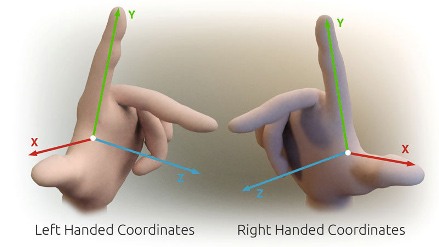
\includegraphics[width=.4\textwidth]{./../Pictures/fig_appendix_A_5.png}
	\figcaption{右手坐标系和左手坐标系。 Figure by Primalshell (Wikimedia Commons) released under a CC-BY-SA-3.0 licence: \url{http://creativecommons.org/licenses/by-sa/3.0/deed.en}. URL:\url{http://commons.wikimedia.org/wiki/File:3D_Cartesian_Coodinate_Handedness.jpg}, Accessed: 1.12.2014}
}

我们无法将一个左手系旋转成一个右手系。事实上,这两类坐标系通过镜面反射相关联。这就是说,右手系和左手系由如下形式的变换相联系%
\footnote{译注:原文这里给出的其实是一个相对原点的反射,而不是镜面反射。当然,这两种反射之间只差一个转动。}
\begin{equation}
\begin{pmatrix}
v_1 \\ v_2 \\ v_3
\end{pmatrix} \rightarrow
\begin{pmatrix}
-v_1 \\ -v_2 \\ -v_3
\end{pmatrix}\text{,}
\end{equation}
就是说把全部空间坐标都反一个号。人们也习惯于将这类变换称作{\bf 宇称变换(parity transformation)}。我们可以用如下方式来表示一个宇称变换
\begin{equation}
\vec{v} \rightarrow \vec{v}' = P\vec{v} = \begin{pmatrix}
-1 & 0 & 0 \\ 0 & -1 & 0 \\ 0 & 0 & -1
\end{pmatrix}
\begin{pmatrix}
v_1 \\ v_2 \\ v_3
\end{pmatrix} =
\begin{pmatrix}
-v_1 \\ -v_2 \\ -v_3
\end{pmatrix}\text{。}
\end{equation}

\chapter[微积分]{Calulus 微积分}\label{appendix.B}

\section[Product Rule]{Product Rule 莱布尼兹律}\label{appendix.B.1}
莱布尼兹律\footnote{译注:直译为“乘积规则”,鉴于这种叫法在中文文本中较罕见,故译作“莱布尼兹律”。}
\begin{equation}
\frac{\rd}{\rd x} \left(f(x)g(x)\right) = \left(\frac{\rd f(x)}{\rd x}\right) g(x) + f(x) \left(\frac{\rd g(x)}{\rd x}\right) \equiv f'g + fg'
\label{equB.1}
\end{equation}
可直接由导数的定义得到
\begin{equation*}
\begin{aligned}
\frac{\rd}{\rd x} \left[f(x)g(x)\right] &= \lim_{h\rightarrow 0} \frac{f(x+h)g(x+h)-f(x)g(x)}{h} \\
 &= \lim_{h\rightarrow 0} \frac{\left[f(x+h)g(x+h)-f(x+h)g(x)\right]+\left[f(x+h)g(x)-f(x)g(x)\right]}{h} \\
 &= \lim_{h\rightarrow 0}{f(x+h)\frac{g(x+h)-g(x)}{h} +g(x)\frac{f(x+h)-f(x)}{h}} \\
 &= f(x)g'(x)+g(x)f'(x)
\end{aligned}
\end{equation*}
\section[分部积分]{Integration by Parts 分部积分}\label{appendix.B.2}
\begin{quote}
据说, Peter Lax 被授予美国国家科学奖章时,其他获奖人(可能不是数学家)问他凭借什么拿到的这个奖。 Lax 回答:“我做了个分部积分。” \\
- Willie Wrong\mpar{是他在\url{www.math.stackexchange.com}上说的。}
\end{quote}

从莱布尼兹律可以直接得到一个重要的积分手段。将莱布尼兹律一式积分%
\mpar{见\eqref{equB.1}式,并利用微积分基本定理$\int_a^b h'(x)=h(b)-h(a)$。}
\begin{equation}
\underbrace{\int_a^b \rd x\, \frac{\rd}{\rd x}\left(f(x)g(x)\right)}_{=\left.f(x)g(x)\right|_a^b} = \int_a^b\rd x\, \left(\frac{\rd f(x)}{\rd x}\right)g(x) + \int_a^b\rd x\, f(x)\left(\frac{\rd g(x)}{\rd x}\right)
\end{equation}
移项,得到
\begin{equation}
\int_a^b \rd x\, \left(\frac{\rd f(x)}{\rd x}\right)g(x) = \left.f(x)g(x)\right|_a^b - \int_a^b\rd x\, f(x)\left(\frac{\rd g(x)}{\rd x}\right)\text{。}
\label{equB.3}
\end{equation}
当讨论场的物理时,这个手段很是有用:在全空间作积分时,即$a=-\infty,b=\infty$,由于一切场量在无穷远处都必须为零%
\mpar{\ref{sec2.4}节中我们说到了没什么能比光速还快,故无穷远处的场一定不会对有限$x$处的物理产生影响。}%
,边界项为零$\left.f(x)g(x)\right|_a^b=0$。

\section[Taylor 级数]{The Taylor Series\quad Taylor 级数}\label{appendix.B.3}
Taylor 级数使我们能将任何无穷阶可微函数写成幂级数形式
\begin{equation}
f(x) = f(a) + (x-a)f'(a) + \frac{1}{2}(x-a)^2f''(a)+\dots
\end{equation}
\begin{itemize}
\item 一方面我们能用它来求某些函数的级数形式。这可以用来,例如,说明$\ue^{\ri x}=\cos (x)+\ri\sin (x)$。
\item 另一方面,也能用它来得到函数在某点附近的近似值。当出于某些原因我们可以略去高阶项,不用考虑无穷多项时,这公式的用处会很大。比如说我们要算函数$f(x)$在$y$的邻域中一点$y+\Delta y$的值,可以写出%
\mpar{不要被这些变量的名字搞混了。上面的公式里我们是从$a$出发计算函数在$x$处的值。而这里我们是希望利用$y$处的信息来得到$f$在$y+\Delta y$处的性质。准确的关系是:$x=y+\Delta y$和$a=y$。}
\end{itemize}
\begin{equation}
f(y+\Delta y) = f(y)+(y+\Delta y-y)f'(y)+\dots =f(y)+\Delta y f'(y)+\dots
\end{equation}
这就是说,通过在$y$处函数的性质,我们能得到其在$y+\Delta y$处的近似值。对于无穷小邻域%
\footnote{译注:原文有误,已更正。}%
$\Delta y=\epsilon\rightarrow 0$的极端情况,函数的改变量可以仅用 Taylor 级数的一(线性)项来表示
\begin{equation}
\Delta f =f(y+\epsilon)-f(y)=f(y)+\epsilon f'(y)+\dots -f(y)=\epsilon f'(y) + \underbrace{\dots}_{\mathclap{\approx 0\text{由于}\epsilon^2\approx 0}}
\end{equation}

这个式子是最有用的数学工具之一,它也能通过微积分基本定理和分部积分推出来。基本定理说
\begin{equation}
\int_a^x\rd t\, f'(t) = f(x) - f(a) \rightarrow f(x)=f(a)+\int_a^x\rd t\, f'(t)\text{。}
\end{equation}
可以将第二项用分部积分写开:在$f'(t)$前面补一个$1$成$1f'(t)$,利用\eqref{equB.3}式取$g'(t)=1$的情况。分部积分能改写积分%
\mpar{译注:原文有误,已更正。}%
$\int_a^b v'u = \left.vu\right|_a^b-\int_a^b vu'$,积掉一项而对另一项微分。这里我们积$g'(t)=1$而微分$f'(t)$,即式子里$g'=v'$及$f'=u$。求得
\begin{equation}
f(x) = f(a)+\int_a^x\rd t\, f'(t) = f(a) + \left.g(t)f(t)\right|_a^x - \int_a^b \rd t g(t)f''(t) \text{。}
\end{equation}

现在的问题是$g(t)$是啥。我们目前只知道$g'(t)=1$,但却有无穷多个函数的导数都是这个:对于任意常数$c$,函数$g=t+c$都满足$g'(t)=1$。我们选取%
\mpar{方程对任意$c$都成立,我们自然可以随便选一个,但那样就推不出我们想要的公式了。选取恰当的$c$是为了得到一个有用的关于$f(x)$的公式。否则$f(x)$将会同时出现在等式两侧。}%
$g=t-x$,即将积分上界的负值$-x$作为我们的常数$c$。从而上式的第二项就可以写作
\begin{equation}
\left.g(t)f(t)\right|_a^x = \left.(t-x)f(t)\right|_a^x = \underbrace{(x-x)}_{=0}f(x) -(a-x)f(a) =(x-a)f(a)
\end{equation}
从而整个式子现在写作
\begin{equation}
f(x) = f(a) + (x-a)f'(a)+\int_a^x\rd t\, (x-t)f''(t)\text{。}
\end{equation}
对最后一项再次使用分部积分,现在是%
\mpar{注意$v='(x-t)$对$t$的积分会出一个符号:$v=-(x-t)^2+d$积分常数$d$取作零。}
$v'=(x-t)$和$u=f''(t)$:
\begin{equation*}
\rightarrow \int_a^x \rd t\, \underbrace{(x-t)}_{\mathclap{=v'}}\underbrace{f''(t)}_{=u} = \left.\underbrace{-\frac{1}{2}(x-t)^2}_{=v} \underbrace{f''(t)}_{=u}\right|_a^x - \int_a^x \rd t\, \underbrace{\left(-\frac{1}{2}(x-t)^2\right)}_{=v}\underbrace{f'''(t)}_{=u'}
\end{equation*}
边界项同样简单的是零
\begin{equation*}
\left.-\frac{1}{2}(x-t)^2f''(t)\right|_a^x = -\frac{1}{2}\underbrace{(x-x)^2}_{=0}f''(x) + \frac{1}{2}(x-a)^2f''(a)\text{。}
\end{equation*}
得到公式
\begin{equation}
f(x)=f(a)+(x-a)f'(a)+\frac{1}{2}(x-a)^2f''(a)+\int_a^x \rd t\, \frac{1}{2}(x-t)^2 f'''(t)\text{。}
\end{equation}
可以继续将最后一项分部积分,但是我们应该能直接肉眼观察出规律了。Taylor 级数可以利用求和号$\Sigma$写成更紧凑的形式:
\begin{equation}
\begin{aligned}
f(x) =& \sum_{n=0}^\infty\frac{f^{(n)}(a)(x-a)^n}{n!} \\
 =& \frac{f^{(0)}(a)(x-a)}{0!} + \frac{f^(1)(a)(x-a)^1}{1!} + \frac{f^{(2)}(a)(x-a)^2}{2!} \\
 =& \frac{f^{(3)}(a)(x-a)^3}{3!}+\dots \text{,}
\end{aligned}
\label{equ.appendix.B.12}
\end{equation}
其中$f^{(n)}$代表$f$的$n$阶导数,例如$f^{(2)}=f''$,$n!$代表$n$的阶乘,即$n!=1\cdot 2\cdot 3\dots n$。比如对$n=5$有$5!=5\cdot 4\cdot 3\cdot 2\cdot 1=120$,$2!=2\cdot 1=2$,以及定义$0!=1$。级数是下一节的主题。
\section[级数]{Series 级数}\label{appendix.B.4}
上一节中我们碰巧发现了含有无穷求和的一个重要等式。在这一节里将介绍关于求和的一些小技巧和几个重要级数。
\subsection[几个重要的级数]{Important Series 几个重要的级数}\label{appendix.B.4.1}
从上一节中我们学到了任意无穷可微的函数都可以写成级数的形式%
\footnote{译注:一个典型的反例是$f(x)=\exp(-1/x^2)$,它在原点处(补充定义后)任意阶导数都为零。}%
。让我们从最重要的例子开始:指数函数$\ue^{x}$。它的泰勒展开式可以直接写出:
\begin{equation}
\ue^x  = \sum\limits_{n=0}^{\infty} \frac{x^n}{n!} \text{,}
\end{equation}
用到了指数函数的%
\footnote{译注:某一种}
定义,导函数等于自身:$(\ue^x)'=\ue^x$。将$a=0$带入 Taylor 级数,利用$\ue^0=1$,便得到指数函数的 Taylor 级数(\eqref{equ.appendix.B.12}式):
\begin{equation}
\ue^x = \sum\limits_{n=0}^\infty \frac{\ue^0(x-0)^n}{n!} = \sum\limits_{n=0}^\infty \frac{x^n}{n!}
\end{equation}

这个级数也可以作为$\ue^x$的定义式。

另外两个无穷可微的重要函数是$\sin(x)$和$\cos(x)$。利用$(\sin(x))'=\cos(x)$,$(\cos(x))'=-\sin(x)$,$\cos(0)=1$以及$\sin(0)=0$,可以推得它们的泰勒级数。
\begin{equation*}
\sin(x) = \sum\limits_{n=0}^\infty \frac{\sin^{(n)}(0)(x-0)^n}{n!}\text{。}
\end{equation*}
由于$\sin(0)=0$,故全部偶数$n$项都为零,由此可以将求和分开:注意到
\begin{equation}
\begin{aligned}
\sum_{n=0}^{\infty}n &= \sum_{n=0}^\infty (2n+1) + \sum_{n=0}^\infty (2n) \\
1+2+3+4+5+6\dots &= 1+3+5\dots + 2+4+6+\dots
\end{aligned}
\end{equation}
将$\sin(x)$的求和分裂开来
\begin{equation}
\begin{aligned}
\sin(x) &= \sum\limits_{n=0}^\infty \frac{\sin^{(2n+1)}(0)(x-0)^{2n+1}}{(2n+1)!}+ \underbrace{\sum\limits_{n=0}^\infty \frac{\sin^{(2n)}(0)(x-0)^{2n}}{(2n)!}}_{=0} \\
 &= \sum\limits_{n=0}^\infty \frac{\sin^{(2n+1)}(0)(x-0)^{2n+1}}{(2n+1)!}\text{。}
\end{aligned}
\label{equ.appendix.B.16}
\end{equation}
$\sin(x)$的全部偶数阶导数,$\sin^{(2n)}$也是$\sin(x)$(除去可能有的负号),由于$\sin(0)=0$所以说第二项为零。$\sin(x)$全部奇数阶导数是$\cos(x)$,除去可能的负号。我们有
\begin{equation}
\begin{aligned}
\sin(x)^{(1)}&=\cos(x) \\
\sin(x)^{(2)}&=\cos'(x)=-\sin(x) \\
\sin(x)^{(3)}&=-\sin'(x)=-\cos(x) \\
\sin(x)^{(4)}&=-\cos'(x)=\sin(x) \\
\sin(x)^{(5)}&=\sin'(x)=\cos(x) \\
\end{aligned}
\end{equation}
规律是$\sin^{(2n+1)}(x)=(-1)^n\cos(x)$,你可以将任意整数$n$带入验证%
\mpar{\begin{align}
\sin(x)^{(1)}=&\sin(x)^{(2\cdot 0+1)}\nonumber \\
&=(-1)^0\cos(x)\nonumber \\
&=\cos(x),\sin(x)^{(3)}\nonumber \\
&=\sin(x)^{(2\cdot 1+1)}\nonumber \\
&=(-1)^1\cos(x)\nonumber \\
&=-\cos(x)\nonumber
\end{align}}%
。由此将\eqref{equ.appendix.B.16}式改写作
\begin{equation}
\begin{aligned}
\sin(x) &= \sum\limits_{n=0}^{\infty}\frac{\sin^{(2n+1)}(0)(x-0)^{2n+1}}{(2n+1)!} \\
&= \sum\limits_{n=0}^{\infty}\frac{(-1)^n\cos(0)(x-0)^{2n+1}}{(2n+1)!} \\
&\underbrace{=}_{\cos(0)=1} \sum\limits_{n=0}^\infty \frac{(-1)^n(x)^{2n+1}}{(2n+1)!}
\end{aligned}
\label{equ.appendix.B.18}
\end{equation}
这就是$\sin(x)$的 Taylor 级数,也可以作为$\sin(x)$的定义式。类似的,我们可以得到
\begin{equation}
\cos(x)= \sum\limits_{n=0}^{\infty}\frac{(-1)^n(x)^{2n}}{(2n)!}\text{,}
\label{equ.appendix.B.19}
\end{equation}
其奇数阶导数都正比于$\sin(0)=0$。

\subsection[分裂求和]{Splitting Sums 分裂求和}\label{appendix.B.4.2}
上一节中我们提到了一个有用的计算技巧。那儿我们用了下面这个例子
\begin{equation}
\begin{aligned}
\sum\limits_{n=0}^{\infty}n &= \sum\limits_{n=0}^\infty (2n+1) + \sum\limits_{n=0}^\infty (2n) \\
1+2+3+4+5+6\dots &= 1+3+5\dots + 2+4+6+\dots
\end{aligned}
\end{equation}
来表明我们可以将任何求和分解成偶数和奇数项。$2n$总是偶数,而$2n+1$总是奇数。在上一节中我们就看到了这很有用,但现在可以再看看另一个例子。如果将带有复变量$\ri x$的指数函数的级数分裂开来会怎样?
\begin{equation}
\begin{aligned}
\ue^{\ri x}= &\sum\limits_{n=0}^\infty \frac{(\ri x)^n}{n!}\\
 =& \sum\limits_{n=0}^\infty \frac{(\ri x)^{2n}}{(2n)!}+\sum\limits_{n=0}^\infty \frac{(\ri x)^{2n+1}}{(2n+1)!}
\end{aligned}
\end{equation}
用$(\ri x)^{2n}=\ri^{2n}x^{2n}$和$\ri^{2n}=(\ri^2)^n=(-1)^n$来写开。另外也需要$\ri^{2n+1}=\ri\cdot \ri^{2n}=\ri(-1)^n$。由此有
\begin{equation}
\begin{aligned}
\ue^{\ri x}= &\sum\limits_{n=0}^\infty \frac{(\ri x)^n}{n!}\\
 =& \sum\limits_{n=0}^\infty \frac{(-1)^n(x)^{2n}}{(2n)!}+\ri\sum\limits_{n=0}^\infty \frac{(-1)^n(x)^{2n+1}}{(2n+1)!}\\
 =& \underbrace{\sum\limits_{n=0}^\infty \frac{(-1)^n(x)^{2n}}{(2n)!}}_{=\cos(x)\text{ 见\eqref{equ.appendix.B.19}式}}+\ri\underbrace{\sum\limits_{n=0}^\infty \frac{(-1)^n(x)^{2n+1}}{(2n+1)!}}_{=\sin(x)\text{ 见\eqref{equ.appendix.B.18}式}}\\
 =& \cos(x)+\ri\sin(x)
\end{aligned}
\end{equation}

\subsection[Einstein 求和约定]{Einstein's Sum Convention\quad Einstein 求和约定}\label{appendix.B.4.3}
物理中经常有求和,老是写大大的求和号$\Sigma$是很烦人的一件事。所以说某个聪明人引入了一个约定,叫 Einstein 求和约定。根据这个约定每当一个指标在某些项中重复出现两次,如同上面的$n$,那么就意味着一个隐藏的求和号。即
\begin{equation}
a_na_n \equiv \sum\limits_n a_nb_n \text{。}
\end{equation}
其他形式的例子
\begin{equation}
a_nb_nc_m \equiv \sum\limits_n a_nb_nc_m \text{。}
\end{equation}
\begin{equation}
a_mb_nc_m \equiv \sum\limits_m a_mb_nc_m \text{。}
\end{equation}
但是
\begin{equation}
a_nb_m \ne \sum\limits_n a_nb_m\text{,}
\end{equation}
因为一般而言$n\ne m$。没有同伴的指标叫做{\bf 自由指标(free index)},而有同伴要求和的叫做{\bf 哑指标(dummy index)}。具体原因会在下一节中解释。

在$a_nb_nc_m \equiv \sum\limits_n a_nb_nc_m$一例中,$n$是哑指标,而$m$是自由指标。对于$a_mb_nc_m \equiv \sum\limits_m a_mb_nc_m$,指标$m$是哑的而$n$是自由的。
\section[指标记号]{Index Notation 指标记号}\label{appendix.B.5}
\subsection[哑指标]{Dummy Indices 哑指标}\label{appendix.B.5.1}
一定要注意到的一点是,有伴的指标事实上什么用处都没有。将$n$重命名为$k$,什么事都不改变%
\mpar{当然我们不能将一个指标改成另一{\bf 类}指标。例如,我们可以将改$i\rightarrow j$但不能改$i\rightarrow \mu$,因为$\mu$这样的希腊字母指标总是从$0$加到$3$,而$i$这样的罗马数字指标是从$1$加到$3$。}%
,即$n$已经被缩并掉了
\begin{equation}
a_n b_n c_m = a_k b_k c_m \equiv \sum\limits_n a_nb_nc_m \equiv \sum\limits_k a_kb_kc_m \text{。}
\end{equation}
另一方面,自由指标却不能自由的被重命名。将$m$改写作$q$会造成区别,因为等式另一端也必须有相同的自由指标。这就是说当我们单独考察类似于$a_nb_nc_m$这样的项时,总需要将其他带有自由指标$m$的项拉进来,指标要改名就得一起改名。我们来看一个例子
\begin{equation}
F_i = \epsilon_{ijk}a_jb_k\text{。}
\end{equation}
这里除了一个新东西$\epsilon_{ijk}$,带着多个指标,我们暂且不去管它,待会儿会仔细讨论。这里我们能将$\epsilon_{ijk}a_jb_k$的指标$j,k$随意重命名,因为它们被缩并掉了。例如$j\rightarrow u$,$k\rightarrow z$,这样得到$\epsilon_{iuz}a_ub_z$和之前的完全是一样的。另一头,$i$就不是一个哑指标了,我们不能将其重命名$i\rightarrow m$:$\epsilon_{muz}a_ub_z$,因为这样的话上式就会变成
\begin{equation}
F_i = \epsilon_{muz}a_ub_z \text{。}
\end{equation}
再看之前那句话这就显得有点迂腐了,因为很明显得将$F_i$里的$i$改掉来得到一个有意义的等式。但一般来说我们都会单独的讨论一个对象,那就得清楚我们不能去改变哪些东西。
\subsection[带多个指标的对象]{Objects with more than One Index 带多个指标的对象}\label{appendix.B.5.2}
现在可以谈谈那些有多个指标的对象。带两个指标的自然就是矩阵了。第一个指标告诉我们变量是在哪一行而第二个指标代表哪一列。例如
\begin{equation}
M_{ij} \equiv \begin{pmatrix}
M_{11} & M_{12} \\ M_{21} & M_{22}
\end{pmatrix}\text{。}
\end{equation}
对于$M_{12}$就是在第一行第二列。

利用指标可以简单的写出矩阵乘法。两个矩阵的乘积是
\begin{equation}
MN = (MN)_{ij} = M_{ik}N_{kj}\text{。}
\end{equation}

在左边是矩阵乘积$(MN)$的$i$行$j$列的元素,可以由$M$的第$i$行和$N$的第$j$列相乘得到。指标$k$出现了两次,代表一个隐含的求和。有时我们会给一个对象两个或更多的指标(张量)。在这本书中,两个一般就够用了,唯一的例外将在下面几节中讨论到。

\subsection[对称/反对称指标]{Symmetric and Antisymmetric Indices 对称/反对称指标}\label{appendix.B.5.3}
一个矩阵被称为是对称的,若$M_{ij}=M_{ji}$。对于二维情形来说就是$M_{12}=M_{21}$,一个对称矩阵的例子如下
\begin{equation}
\begin{pmatrix}
9 & 3 \\ 3 & 17 \\
\end{pmatrix}
\end{equation}
一个矩阵被称为是{\bf 全反对称的(totally antisymmetric)},若$M_{ij}=-M_{ji}$对于{\bf 全体}$i,j$成立。一个示例是
\begin{equation}
\begin{pmatrix}
0 & 3 \\ -3 & 0
\end{pmatrix}
\end{equation}
注意对角元都是零,这是因为$M_{11}=-M_{11}$仅当$M_{11}=0$时成立,对于$M_{22}$也一样。
\subsection[对称和反对称求和]{Antisymmetric $\times$ Symmetric Sums 对称和反对称求和}\label{appendix.B.5.4}
一个重要的事实:当我们将带有完全相同的指标的对称和反对称的对象乘起来求和时,结果为零:
\begin{equation}
\sum\limits_{ij}a_{ij}b_{ij} = 0
\end{equation}
若有$a_{ij}=-a_{ji}$和$b_{ij}=b_{ji}$对于全部$i,j$成立。这个结论很容易看出来:改写
\begin{equation}
\sum\limits_{ij}a_{ij}b_{ij} = \frac{1}{2}\left(\sum\limits_{ij}a_{ij}b_{ij}+\sum\limits_{ij}a_{ij}b_{ij}\right)
\end{equation}
正如之前解释过的,我们能自由的将哑指标重命名$i\rightarrow j$及$j\rightarrow i$,仅对第二项作用
\begin{equation}
\rightarrow \sum\limits_{ij}a_{ij}b_{ij} = \frac{1}{2}\left(\sum\limits_{ij}a_{ij}b_{ij}+\sum\limits_{ij}a_{ji}b_{ji}\right)
\end{equation}
然后利用$b_{ij}$的对称性和$a_{ij}$的反对称性,来翻转第二项中的指标,得到%
\mpar{如果你觉得这是一个无聊的把戏,算几个真实的例子来验证其正确性。}
\begin{equation}
\begin{aligned}
\rightarrow \sum\limits_{ij}a_{ij}b_{ij} &= \frac{1}{2}\left(\sum\limits_{ij}a_{ij}b_{ij}+\sum\limits_{ij}\underbrace{a_{ji}}_{=-a_{ij}}\underbrace{b_{ji}}_{=b_{ij}}\right)\\
 &= \frac{1}{2}\left(\sum\limits_{ij}a_{ij}b_{ij}-\sum\limits_{ij}a_{ij}b_{ij}\right) = 0
\end{aligned}
\end{equation}
\subsection[两个重要的符号]{Two Important Symbols 两个重要的符号}\label{appendix.B.5.5}
第一个是单位矩阵。二维情形下为
\begin{equation}
1= \begin{pmatrix}
1 & 0 \\ 0 & 1
\end{pmatrix}\text{。}
\end{equation}
单位矩阵用指标记号来标记时称 Kronecker 符号$\delta_{ij}$,对任意维度都可由下式定义
\begin{equation}
\delta_{ij} = \begin{cases}
1 & i=j \\
0 & i\ne j
\end{cases}
\end{equation}
Kronecker符号是对称的,有$\delta_{ij}=\delta_{ji}$。

第二个是 Levi-Civita 符号$\epsilon_{ijk}$,在二维下由下式定义
\begin{equation}
\epsilon_{ij} = \begin{cases}
1 & (i,j)={(1,2)} \\
0 & i=j \\
-1 & (i,j)={(2,1)}
\end{cases}
\end{equation}
矩阵形式写作
\begin{equation}
\epsilon_{ij} = \begin{pmatrix}
0 & 1 \\ -1 & 0
\end{pmatrix}
\end{equation}

三维下的 Levi-Civita 符号是
\begin{equation}
\epsilon_{ijk} = \begin{cases}
1 & (i,j,k)={(1,2,3),(2,3,1),(3,1,2)} \\
0 & i=j\text{或}j=k\text{或}j=i \\
-1 & (i,j,k)={(1,3,2),(3,2,1),(2,1,3)}
\end{cases}
\end{equation}
对于四维
\begin{equation}
\epsilon_{ijkl} = \begin{cases}
1 & \text{若}(i,j,k,l)\text{是}{(1,2,3,4)}\text{的偶置换} \\
-1 & \text{若}(i,j,k,l)\text{是}{(1,2,3,4)}\text{的奇置换}\\
0 & \text{其他}
\end{cases}
\end{equation}
例如$(1,2,4,3)$和$(2,1,4,3)$就分别是$(1,2,3,4)$的奇置换(换了一个)和偶置换(换了两个)。

Levi-Civita 符号是全反对称的:根据定义,当置换两个指标时,总是多一个负号:

$\epsilon_{ijk}=-\epsilon_{jik}$,$\epsilon_{ijk}=-\epsilon_{ikj}$等。或者二维下$\epsilon_{ij}=\epsilon_{ji}$。


%\chapterimage = {
\chapter[线性代数]{Linear Algebra 线性代数}
\label{appendix.C}
利用矩阵等线性代数工具可以大幅简化计算,下面从基本变换开始对线性代数做一回顾。



\section[基本变换]{Basic Transformations 基本变换}
\label{appendix.C.1}
{\bf 矩阵的复共轭}定义为:
\begin{equation}
\label{equc.1}
	M^*_{ij} =
		\begin{pmatrix}
			M^*_{11} & M^*_{12} \\
			M^*_{21} & M^*_{22}
		\end{pmatrix},
\end{equation}
即对每个矩阵元取复共轭%
\mpar{复数$z = a + ib$($a$为$z$的实部,$b$为虚部,$a, b$均为实数)的复共轭为$z^* = a - ib$。}%
。

{\bf 矩阵的转置}定义为$M^T_{ij} = M_{ji}$,用矩阵形式表示为:
\begin{equation}
\label{equC.2}
	M_{ij} =
		\begin{pmatrix}
			M_{11} & M_{12} \\
			M_{21} & M_{22}
		\end{pmatrix}
	\ \to \
	M^T_{ij} =
		\begin{pmatrix}
			M_{11} & M_{21} \\
			M_{12} & M_{22}
		\end{pmatrix},
\end{equation}
即交换矩阵的行与列。两个矩阵的乘积的转置$(MN)^T \neq M^T N^T$,而是$(MN)^T = N^T M^T$,即乘积的转置需要调换乘积顺序,这用指标记号不难证明:
\begin{align}
	MN \equiv (MN)_{ij} = M_{ik} N_{kj} \notag \\
	(MN)^T \equiv \big( (MN)_{ij} \big)^T = (MN)_{ji} = (M_{ik} N_{kj})^T \notag \\
\label{equC.3}
	(M_{ik} N_{kj})^T = M^T_{ik} N^T_{kj} = M_{ki} N_{jk} = N_{jk} M_{ki} \equiv N^T M^T,
\end{align}
其中最后一步利用了矩阵乘法的指标记号,左侧矩阵的行乘以右侧矩阵的列。我们将$M_{ki} N_{jk}$写为$N_{jk} M_{ki}$的形式,后者即为左侧矩阵的行乘以右侧矩阵的列的形式,这样就能用矩阵乘法记作$N^T M^T$.

注意在指标记号下乘积中的各项顺序可自由颠倒,例如$M_{ki} N_{jk} = N_{jk} M_{ki}$,因为各$M_{ki}$与$N_{jk}$只代表数字。


\section[矩阵指数函数]{Matrix Exponential Function 矩阵指数函数}
\label{appendix.C.2}
前面已经导出了指数函数的级数形式,由此可定义矩阵的指数函数$\mathrm{e}^M$,其中$M$为任意方阵:
\begin{equation}
\label{equC.4}
	\mathrm{e}^M = \sum_{n = 0}^\infty \frac{M^n}{n!}.
\end{equation}
必须注意,一般$\mathrm{e}^M \mathrm{e}^N \neq \mathrm{e}^{M + N}$。$\mathrm{e}^M \mathrm{e}^N = \mathrm{e}^{M + N}$当且仅当$MN = NM$.

\section[行列式]{Determinants 行列式}
\label{appendix.C.3}
矩阵行列式的概念不太直观,但是相当有用。例如,若矩阵的行列式非零,则该矩阵可逆%
\mpar{若矩阵$M$可逆,则它存在逆矩阵,记作$M^{-1}$,满足$M^{-1} M = M M^{-1} = \mathbf{1}\text{(单位矩阵)}$.}%
。这个命题的证明有点复杂,读者可在任何一本线性代数教材中查阅。

$3 \times 3$矩阵的行列式$\det (A)$可以用Levi-Civita符号定义:
\begin{equation}
\label{equC.5}
	\det (A) = \sum_{i = 1}^3 \sum_{j = 1}^3 \sum_{k = 1}^3 \epsilon_{ijk} A_{1i} A_{2j} A_{3k},
\end{equation}
$n \times n$矩阵的行列式的定义类似:
\begin{equation}
\label{equC.6}
	\det (A) = \sum_{i_1 = 1}^n \sum_{i_2 = 1}^n \cdots \sum_{i_n = 1}^n \epsilon_{i_1 i_2 \dots i_n} A_{1 i_1} A_{2 i_2} \dots A_{n i_n}.
\end{equation}
例:$2 \times 2$矩阵的行列式
\[
	\det (A) = \det
		\begin{pmatrix}
			3 & 1 \\
			5 & 2
		\end{pmatrix}
	= (3 \cdot 2) - (5 \cdot 1) = 1
\]
一般$3 \times 3$矩阵的行列式:
\begin{equation}
\label{equC.7}
	\det
		\begin{pmatrix}
			a_1 & a_2 & a_3 \\
			b_1 & b_2 & b_3 \\
			c_1 & c_2 & c_3
		\end{pmatrix}
	= a_1 (b_2 c_3 - b_3 c_2) - a_2 (b_1 c_3 - b_3 c_1) + a_3 (b_1 c_2 - b_2 c_1).
\end{equation}


\section[本征值与本征向量]{Eigenvalues and Eigenvectors 本征值与本征向量}
\label{appendix.C.4}
本征值与本征向量是物理学中大用特用的线性代数概念。矩阵$M$的特征值$\lambda$与特征向量$\vec{v}$满足:
\begin{equation}
\label{equC.8}
	M \vec{v} = \lambda \vec{v}.
\end{equation}
上式两侧作用的是同一向量$\vec{v}$,这意味着$\vec{v}$经矩阵$M$变换后只改变原来的常数$\lambda$倍。每一本征向量对应一个本征值。计算本征值与本征向量的过程有点繁复,可以参考任何一本线性代数教材。

本征向量重要性的一个例子是旋转变换,我们用旋转矩阵描述旋转操作,用旋转矩阵的本征向量定义各旋转轴。


\section[对角化]{Diagonalization 对角化}
\label{appendix.C.5}
利用本征值与本征向量可以使矩阵对角化,这能简化计算,并且有助于解释方程的物理意义。可以证明任意可对角化的矩阵$M$能写为如下形式%
\mpar{一般情况,变换$M' = N^{-1} M N$意味着基的变换,$M'$是$M$在新坐标系中的形式。因此矩阵对角化的含义就是可以找到一个坐标系使得矩阵$M$在该坐标系中的形式简单(对角矩阵)。}%
:
\begin{equation}
\label{equC.9}
	M = N^{-1} D N,
\end{equation}
其中矩阵$N$由$M$的本征向量组成,矩阵$D$是以$M$的本征值为对角元的对角矩阵:
\begin{equation}
\label{equC.10}
	\begin{pmatrix}
		M_{11} & M_{12} \\
		M_{21} & M_{22}
	\end{pmatrix}
	= N^{-1}
		\begin{pmatrix}
			\lambda_1 & 0 \\
			0 & \lambda_2
		\end{pmatrix}
	N = \Big( \vec{v}_1, \vec{v}_2 \Big)^{-1}
		\begin{pmatrix}
			\lambda_1 & 0 \\
			0 & \lambda_2
		\end{pmatrix}
	\Big( \vec{v}_1, \vec{v}_2 \Big).
\end{equation}


\chapter[其他数学概念]{Additional Mathematical
Notions \quad 其他数学概念}\label{appendix.D}
\section{Fourier变换}\label{appendix.D.1}
Fourier变换的思想类似于把一个任意向量按照一组基底矢量$(\vec{e_1},\vec{e_2},\vec{e_3})$做展开\footnote{关于后者的详细介绍参见附录A.1},在三维欧氏空间下最常见的基底选择为
\begin{equation}
\vec{e_1}=\pmm 1\\0\\0 \pmme,~~
\vec{e_2}=\pmm 0\\1\\0 \pmme,~~
\vec{e_3}=\pmm 0\\0\\1 \pmme
\end{equation}
任意三维矢量$\vec{v}$可以按这组基底展开为
\begin{equation}
\vec{v}=\pmm v_1\\v_2\\v_3 \pmme =v_1\vec{e_1}+v_2\vec{e_2}+v_3\vec{e_3}=v_1\pmm 1\\0\\0 \pmme+v_2\pmm 0\\1\\0 \pmme +v_3\pmm 0\\0\\1 \pmme
\end{equation}
傅里叶变换的概念就是对函数做类似的展开\footnote{从更抽象的层面来说,函数是广义上的矢量,也就是说它们是一个矢量空间中的元素。对于不同种类的函数它们所组成的矢量空间也是不同的。这种广义矢量空间的定义和通常欧氏矢量空间的类似(后者就是我们常见的带小箭头$\vec{~}$的位置矢量构成的空间),比如说,你可以像加两个向量一样把两个函数加起来,并可以对函数定义标量积。},对于周期函数来说展开的基底是$\sin(kx)$和$\cos(kx)$,也就是说任意周期函数都可以写成如下形式\footnote{在某些点上未必如此,具体取决于函数和边界条件。更详细的介绍可以参见任意一本数学物理方法教材(鉴于大多数读者都是物理系而非数学系的学生)——译者}
\begin{equation}
  f(x)=\sum^{\infty}_{k=0}(a_k\cos(kx)+b_k\sin(kx))
\end{equation}
其中$a_k$和$b_k$为常系数。\par
任意(无需周期条件)函数可以按基底$e^{ikx}$和$e^{-ikx}$展开,但是这时候求和号被积分号代替\footnote{复习一下,积分实际上就是求和的极限过程,$\sum_k$ 中分立变量k在$\int dk$中变成了连续变量。}:
\begin{equation}
  f(x)=\int^\infty_0 dk(a_k e^{ikx}+b_k e^{-ikx})
\end{equation}
我们也可以把上式写成
\begin{equation}
  f(x)=\int^\infty_{-\infty} dk f_k e^{-ikx}
\end{equation}
展开系数$f_k$可以写成$\tilde f(k)$,其常被称为$f(x)$的傅里叶变换。
\section{$\delta$分布函数}\label{appendix.D.2}
从某种角度上来说,$\delta$分布函数在积分中起的作用和Kronecker$\delta$符号
\footnote{Kronecker$\delta$符号定义见附录B.5.5}在求和中起的作用类似。举个例子,考虑
\begin{equation}
  \sum_{i=1}^3 a_i b_j=a_1 b_j+a_2 b_j+a_3 b_j
\end{equation}
现在我们想把求和的第二项提取出来,我们可以利用Kronecker$\delta$符号$\delta_{2i}$,这样得到
\begin{equation}
  \sum_{i=1}^3 \delta_{2i} a_i b_j=\delta_{21} a_1 b_j+\delta_{22} a_2 b_j+\delta_{23} a_3 b_j=a_2 b_j
\end{equation}
写成更一般的式子即为
\begin{equation}
  \int^3_{i=3} \delta_{ik} a_i b_j=a_k b_j
\end{equation}
$\delta$分布函数$\delta(x-y)$由下式定义:
\begin{equation}
    \int dx f(x)\delta(x-y)=f(y)
\end{equation}
和Kronecher$\delta$符号非常类似,$\delta$分布函数从积分中提取出了一项
\footnote{即$x=y$的一项,例如,$\int dx f(x)\delta(x-2)=f(2)$.},我们还可以通过相似性从式
\begin{equation}
  \frac{\partial x_i}{\partial x_j}=\delta_{ij}
\end{equation}
推出
\begin{equation}
    \frac{\partial f(x_i)}{\partial f(x_j)}=\delta(x_i-x_j)
\end{equation}
通过相似性来导出此式当然不能算是一个证明,如果你愿意你也可以通过严格的数学推导得到这个式子。关于$\delta$分布函数还有很多内容可以讲,但就此书的目的而言你只需要知道它是干什么的就足够了。事实上,这也是Dirac最早引入这一函数的方式。
